\chapter{Implementation}
This chapter covers the interesting parts of the implementation of the Vector Screencast project. The following text summarizes the ideas behind the concepts used in the project and problems, that had to be overcome.

\section{ECMAScript and JavaScript}
ECMAScript is a standardized scripting language widely used in website development~\cite{ecmascript}. Latest approved edition of ECMAScript is \textit{ECMAScript 5.1}, which is implemented in most major web browsers. Implementations of ECMAScript in web browsers are commonly called JavaScript. 

JavaScript is a dynamic programming language, which combines multiple aspects of imperative, functional, and object-oriented programming.

Functions are so called first-class citizens. This means they can be stored in variables, passed as function parameters, returned as results of functions, and included in data structures.

JavaScript doesn't provide any means of static type checking. All types are created during runtime and they are also checked only during runtime. The lack of static type checking during compilation might lead to rarely occurring errors and it is important to take this in mind while writing JavaScript code. A good practice is to write documentation comments\footnote{Commonly used syntax in JavaScript projects is JSDoc (http://usejsdoc.org/)}, where the types are stated.

JavaScript is an interpreted language, some implementations also use a \nomenclature{JIT}{Just-In-Time compilation} \textit{Just-In-Time} (JIT) compilation \footnote{For example Google V8 engine used in Google Chrome. See https://code.google.com/p/v8/} for better performance.  Another very important aspect of ECMAScript which affects its performance is the absence of direct control over memory usage -- memory is released when it is not needed any more. This mechanism is called \textit{Garbage collection}. As of 2012, all modern browsers use mark-and-sweep garbage-collector~\cite{mdn_memory_management}.

\textit{Object oriented programming} (OOP)\nomenclature{OOP}{Object oriented programming} in JavaScript differs from class-oriented OOP in the way inheritance is implemented. While in class-oriented languages, for example in C++ or C\#, inheritance is achieved by declaring classes of objects. In JavaScript, OOP is implemented through object prototypes. Prototype is just a link to another object, which has another prototype. A prototype chain is created this way. The last object in this chain has a \verb|null| prototype. When trying to access a property of an object, it is searched in its own properties. If it is not found, then it is searched in its prototype's properties and so on until the end of the prototype chain is reached~\cite{mdn_prototype_chain}.

\subsection{TypeScript}
\textit{TypeScript} is a typed superset of JavaScript that compiles to plain JavaScript\cite{typescript}. It is an open-source project developed by Microsoft. It is, as its name suggests, a strongly typed programming language compatible with JavaScript.

TypeScript extends capabilities of JavaScript by static type checking at the time of compilation, which helps the programmer to find errors in source code sooner, and speeds up the process of coding. TypeScript also introduces \textit{class} semantics. These classes are transpiled into JavaScript prototypes. TypeScript also includes concepts of interfaces and polymorphism, which makes programs written in TypeScript more understandable to programmers familiar with other object-oriented programming languages like Java, C\# or C++.

TypeScript uses several features of ECMAScript 6, but it is transpiled into ECMAScript 5.1, and therefore does not bring any new functionality. The reason for choosing TypeScript is the clarity of code and more convenient development process for the programmer.



\section{Event driven programming}
The idea behind event driven programming is to break direct references between objects and to communicate with \textit{events} instead of calling object methods directly. The advantage of the this approach is the so called \textit{loose coupling}~\cite{loose_coupling} -- features might be added or removed without breaking the core of the application.

Each object handles only its own task without knowing anything about the other objects it is collaborating with. When an object completes its task, it publishes the result with a specific event. Objects subscribed for this event are notified and are given the outcomes of the previous task.

This mechanism is sometimes called the \textit{Event Aggregator} design pattern. It is implemented through the \verb|VideoEvents|\footnote{Implementation can be found in \texttt{/public/js/app/Helpers/VideoEvents.ts} file} static class, which makes it a simple singleton object. This class provides an interface for registering and triggering callbacks for specified events. Callbacks executed by a triggered event are called asynchronously. It is worth mentioning that web browsers execute all scripts in a single thread.

For example of \verb|VideoEvents| usage, see the following example:

\begin{lstlisting}
	var VET = VideoEventType;

	VideoEvents.on(VET.Message, function(message) {
		console.log("received message:", message);
	});

	VideoEvents.on(VET.Message, function(message) {
		console.log("received message backwards:", message.split("").reverse().join(""));
	});

	VideoEvents.trigger(VET.Message, "Hello world.");
\end{lstlisting}


The list of all event types can be found in the enclosed API documentation of the \verb|VideoEventType| enumeration\footnote{The ``Message'' event used in the example is not used in the Vector Screencast project and was used only as an illustration.}.


\section{HTML5}

HTML5 is a term used to refer to modern web technologies. The core is the \textit{HyperText Markup Language}, designed to describe semantics of structured docu ents~\cite{html5}. HTML5 extends the semantics of HTML 4.1 with new HTML tags such as \verb|<header>| or \verb|<footer>|, but also defines a huge set of new APIs, which allow web developers to create much richer websites and web applications. Some of these new technologies are needed by the Vector Screencasts project.

\paragraph{Working with XML documents}
Working with XML data is very similar to working with regular website DOM in JavaScript. \verb|Document| interface is used for traversing the XML tree, modifying it or for creating a new one. In HTML5, XML files can be opened using a HTTP GET request via \verb|XMLHttpRequest|\nomenclature{XHR}{XMLHttpRequest} object, which parses the data and returns a \verb|Document| instance in its \verb|responseXML| property, if the document meets specified criteria~\cite{xhr}.

\paragraph{WebSockets}
WebSockets allow applications to open bidirectional communication channels with server-side processes~\cite{websocket}. WebSockets are built on top of the \textit{Transmission Control Protocol} (TCP)\nomenclature{TCP}{Transmission Control Protocol} connection. This means that the delivery of data is reliable and ordered.

\paragraph{Web Workers}
JavaScript code of a website normaly runs in a single thread. It is common to run functions asynchronously, for example callback functions and event handlers, but all these functions still run in the same thread. Web Workers are a means of running heavy tasks in background without affecting the user interface. A real OS-level \nomenclature{OS}{Operating system} thread is spawn for each \verb|Worker| object instance.

Web Workers have several limitations. They cannot change the DOM and have direct links to objects in the main thread. Web workers receive messages from the parent thread through an \verb|onmessage| event and can send a response via the \verb|postMessage| function. These messages contain serialized JavaScript objects, which cannot contain any references. As a result, concurrency problems are not typically an issue. Web Workers can perform HTTP requests using the \verb|XMLHttpRequest| object, but the content is not parsed, if the target is an XML or HTML file. For more details see the specification of the Worker object.



\section{Screencast playback}
The screencast player uses a ``stopwatch'' -- high resolution timer -- to keep track of current video time. The key job of the screencast player is to synchronize the state of the canvas with the state of the recorded video according to current time.

The simplest way to synchronize the video is to sequentially execute video commands, whose timestamp is lesser or equal to current time. This process must be repeated periodically whenever the video is started or unpaused. The optimal frequency of an animation is 60~Hz. This frame rate can be targeted by periodically running the \verb|requestAnimationFrame| method.

Executing commands consequently will become ineffective, when the user skips to a random part of the video. Naive implementation would set the timer to the chosen time and for a point in the future, execute all the commands, until the states are synchronized. For a point in the past, the blackboard would be cleared and the initial state will be synchronized with the state at the chosen time.

This approach can be optimalised by looking at the last time, when the board was cleared the last time before the chosen time. Synchronization must then start at this point. This means looking up the chunk, into which the time steps, and looking up the very previous ``erase'' chunk. This can be done at the time of parsing the screencast input file.

Each chunk represents a graphical primitive and can be rendered at once. This can be used to render all the chunks but the last one during the synchronization. The commands for changing current brush size and current brush color are skipped, therefore each chunk must remember only the color and brush size at the moment of its start of processing.

Most of the commands are cursor movement commands -- cursor is moved only to its final position during one synchronization step. This reduces extra triggered events.






\section{Drawing lines}
Khan Academy videos are known for their consistent and simple style. A person draws on a virtual canvas (evoking a school blackboard) with a brush (or possibly a chalk) of a round shape.

Tutor has a pointing device, typically a computer mouse or a digital stylus, and its position on the canvas is marked with a moving cursor. When the tutor clicks, a dot is marked on canvas in the current position of the cursor. Tutor can produce a line (typically a curve) following this cursor when he presses a mouse button or increases digital stylus pressure while moving the cursor. The curve ends when he releases the button or lowers stylus pressure. The color and size of the dot or line corresponds to current settings. Pressed mouse button corresponds to maximal applied pressure and released mouse button to no pressure.

Rendering at the time of playback gives us the opportunity to adjust the outcome to the environment of the end user. This means that the result can be sharp on every display resolution without the need of having many versions of the same video for each resolution.


\subsubsection{Rendering graphics using HTML5}

Displaying text and static visual content is the main purpose of older versions HTML and \textit{Cascade Style Sheets} (CSS)\nomenclature{CSS}{Cascade Style Sheets}. Creating complex polygons or curves would be very hard, involve various tricks \footnote{For example icon shapes can be created using pure CSS: http://nicolasgallagher.com/pure-css-gui-icons/} or would be even impossible. 

The new HTML specification takes this in mind and brings ways of creating more rich and dynamic content within a web page. There are two technologies that should be taken into account -- \textit{Canvas 2D Context} and \textit{SVG}.

\paragraph{Canvas 2D Context}
The \verb|<canvas>| element provides scripts with a resolution-dependent bitmap canvas, which can be used for rendering graphs, game graphics, or other visual images on the fly~\cite{html5_canvas}. 

Using canvas seems appropriate for this project. Canvas could be created with respect to user's resolution and web browser window size. All elements can be scaled to fit this viewport. This will make them look sharp and there will not be any artefacts, noise and blur caused by interpolation used for scaling regular bitmap video content.

When the dimensions of the \verb|<canvas>| element change, the image is scaled, but the output will not be very sharp. Canvas contains a bitmap image, onto which the graphics primitives are drawn. All these primitives must be redrawn by the programmer to achieve smooth scaling.

\paragraph{SVG}
SVG can be used for animation inside a website by adding the \verb|<svg>| element to the DOM. SVG elements are then added, deleted, and modified like any other DOM content. When the content of the SVG element changes or some attributes of SVG elements change, image is redrawn automatically. SVG content is also scaled automatically when the size of the root \verb|<svg>| element changes. It is important to set correct value of \verb|viewBox| attribute. The value should correspond to the size of the original canvas.

\paragraph{WebGL}
\textit{WebGL} is a JavaScript API for rendering 3D and 2D graphics in a webpage. It is based on OpenGL ES 2.0. Vertex and fragment shader code written in HLSL is executed directly on user's Graphics Processing Unit (GPU).


\subsection{Drawing strategy}
There are several methods of rendering graphics in HTML5. Two of them -- Canvas 2D Context and SVG -- are implemented in the Vector Screencasst library. They are not hard-coded into the \verb|{Player| or \verb|Recorder|. User can specify the strategy he wants to use when he creates the object of the tool. The Canvas 2D Context is the default drawing strategy.

If someone wants to use a different rendering method, for example \textit{WebGL}, or rewrite one of the already implemented strategies, he or she might write an own class, which would implement the \verb|{DrawingStrategy| interface and a class extending the \verb|{Path| class. One could use this rendering method in his project without modifying the source code of the library.

Drawing strategy receives segments, which were generated by the Dynadraw algorithm earlier, and renders them with current color. Both ends of a line are ended with a rounded cap.


\subsection{Dynadraw algorithm}
\label{sec:dynadraw}

Paul Haeberli has created a simple algorithm called \textit{``Dynadraw''} in 1989, which is suitable for calligraphy. Brush is modeled as a physical object with its \textit{mass}, \textit{velocity} and \textit{friction coefficient}~\cite{dynadraw}. Mouse movement is interpreted as a way of exerting force on the brush -- the faster you move the brush, the greater the force applied on the brush is. Acceleration is then calculated according to Newton's second law of motion considering brush's mass and velocity of the brush is derived with respect to the value of friction coefficient. This velocity is then applied and brush is moved. The trace brush should leave behind is then drawn onto the virtual canvas.

The advantage of this algorithm is its simplicity and the possibilities of configuring the brush with different values of mass and friction (the author of the algorithm refers to this constant also as \textit{drag}, which better fits the purpose of slowing down the brush).

Heavier brushes move slower than the light ones, but the path they leave behind is much smoother, as the hand shaking is eliminated by composition of forces in different directions.

Light brushes move faster and are often very close to the cursor during the movement. When the cursor stops abruptly, light brushes with little friction tend to keep moving past the cursor and wrap around it. This produces little curls at the end of lines.

\subsubsection*{Brush movement simulation}

One step of simulation applies force on the brush according to current mouse position and thus moves it in the direction of the cursor. This process of applying force must be done periodically, at the frequency of 60~Hz in ideal case\footnote{HTML5 provides \text{requestAnimationFrame} function, which is intended for animations and which targets 60 frames per second}. Implementation of this simulation is not identical to the original \textit{Dynadraw} algorithm, but all of its key aspects are preserved. Pseudocode~\ref{alg:one-step} describes the algorithm used in this thesis.

Even though it is intuitive to measure elapsed time between two steps and correct brush movement using this time difference, this aspect did not yield good results. When the frequency of \verb|requestAnimationFrame| dropps, user's cursor moves further from the previous point, and the force applied on the brush is bigger. Correcting the force caused the brush to wiggle around the cursor wildly.

It turned out to be sufficient to apply the force as much frequently as possible, targeting 60~Hz, but not to calculate speed based on elapsed time. Animation of a line drawing recorded at lower frequency feels less smooth and the line lags behind the cursor more distinctive, than at the ideal frequency. Even though, the result looks subjectively better and more consistent than with time corrections.

The main difference between the original implementation and the one used in Vector Screencast project is brush width calculation. The original algorithm calculates the width of the line in a specific point by measuring its velocity -- the faster the brush is moving, the thinner the drawn line is. This width dynamics gave the algorithm its name.

In our implementation, this effect is preserved, but it is much more subtle. It can be disabled entirely, if the user does not want this feature. Brush dynamics relies mainly on the pressure of a digital stylus on a graphics tablet. Since the exact value of pressure in the point of current brush's location is not always known, the value is linearly interpolated between the value of pressure in the previous position of the brush and the value of pressure in the current mouse position according to the distance from each of these points.

As this simulation is not deterministic, this process cannot be reconstructed afterwards. When the video is being played, only the precomputed values of path segments must be used. The precise value of pressure is therefore irrelevant for later playback of the screencast and does not have to be stored. The advantage of storing this values is the possibility of reconstructing the process of recording later and rendering the lines again. Even a different algorithm might be used in this case.

\begin{pseudocode}
  \begin{algorithmic}

  	\Function{OneStep}{$M$} \Comment $M$ - mouse position
      \If {$M \neq \emptyset$}
	      \State $brushMoved \gets \Call{apply}{\vec{M}} $
          \If {$brushMoved = true$}
              \State \Call{DrawSegment}{}
          \EndIf
      \EndIf
 	\EndFunction

	\Function{apply}{$M$}
      \State $ \vec{F} \gets M - P $\Comment $P$ - current position of the brush
      \State $ \vec{a} = \frac{\vec{F}}{m} $\Comment $m$ - mass of the brush

      \If{$ \norm{\vec{a}} \le C_a $} \Comment $C_a$ - minimum acceleration constant
	      \State \Return false;    
       \EndIf
      
      \State $\vec{v} \gets \vec{v} + \vec{a}$

      \If {$ \norm{\vec{v}} > C_v$} \Comment $C_v$ - minimum velocity constant
          \State $ P \gets P + \mu\vec{v} $\Comment $\mu$ - coefficient of friction
		  \State \Return true
      \EndIf
      \State \Return false
  	\EndFunction
  \end{algorithmic}
\caption{One step of brush movement simulation}
\label{alg:one-step}
\end{pseudocode}

\subsubsection*{Rendering of one line segment}

Line consists of many segments that are drawn after every simulation step, which moves the brush. There are several ways to draw the segment. The most straightforward is to draw a simple quadrilateral as shown in figure~\ref{fig:draw-segment-quadrilateral} and pseudocode~\ref{alg:draw-segment-quadrilateral}.

\begin{pseudocode}
	\begin{algorithmic}
    	\Function{DrawSegment}{}
              \State $ \vec{n} \gets \frac{(-\vec{v}_y, \vec{v}_x)}{\norm{\vec{v}}} $        
              \State $ w \gets \Call{CurrentBrushPressure}{} \cdot b $ \Comment $b$ - brush size
              \State $L \gets P - w\vec{n}$
              \State $R \gets P + w\vec{n}$

              \State \Call{BeginPath}{}
              \State \Call{MoveTo}{$L'$} \Comment $L'$ and $R'$ - previousely drawn point
              \State \Call{LineTo}{$R'$}
              \State \Call{LineTo}{$R$}
              \State \Call{LineTo}{$L$}
              \State \Call{ClosePath}{}
              \State \Call{Fill}{c} \Comment c - current brush color

              \State $L' \gets L$
              \State $R' \gets R$
          \EndFunction
       \end{algorithmic}
  	   \caption{Draw one segment of a line\label{alg:draw-segment-quadrilateral}}      
   \end{pseudocode}

   
  \begin{figure}
  	\centering
      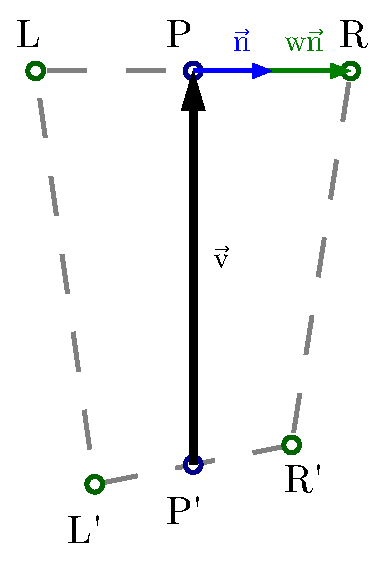
\includegraphics[height=50mm]{../img/draw-segment-quadrilateral.eps}
      \caption{Drawn quadrilateral segment of a line\label{fig:draw-segment-quadrilateral}}      
  \end{figure}


\begin{figure}
	\centering
  		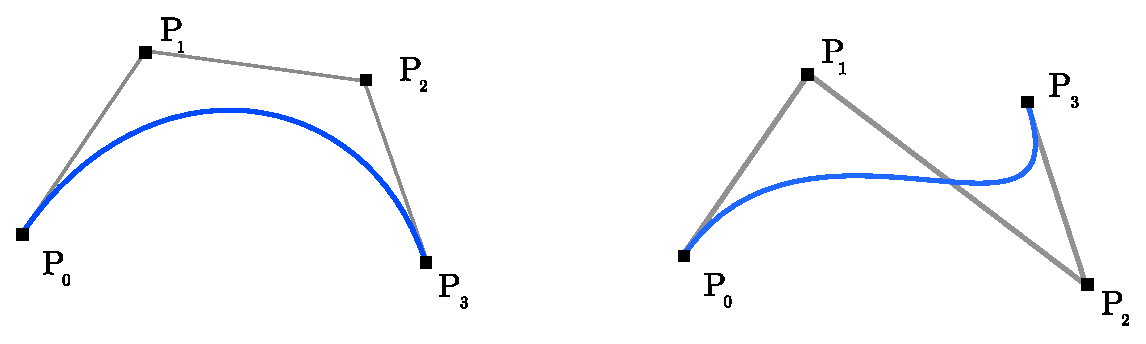
\includegraphics[width=130mm]{../img/bezier_curves.eps}
  		\caption{Bézier curve interpolation examples\label{fig:bezier-curve}}  		
\end{figure}

The curves drawn using quadrilaterals are not very smooth. For smoother curves, straight lines must be replaced with interpolation splines. Both SVG and Canvas 2D Context implement \textit{cubic Bézier curves}. Cubic Bézier curves are defined by four control points, $ \mathbf{P}_0, \mathbf{P}_1, \mathbf{P}_2, \mathbf{P}_3 $. Path starts in $ \mathbf{P}_0 $ and ends in $ \mathbf{P}_3 $, it does not usually go through points $ \mathbf{P}_1, \mathbf{P}_2 $. The interpolation forumla of the curve~\cite{bezier} is

$$ \mathbf{B}(t) = (1 - t)^3 \mathbf{P}_0 + 3(1-t)^{2}t\mathbf{P}_1 + 3(1-t)^{2}t^2\mathbf{P}_2 + t^3\mathbf{P}_3,\quad 0 \leq t \leq 1$$ 

To calculate the control points of a cubic Bézier curve for segment between points $\mathbf{X}_i$ and $\mathbf{X}_{i+1}$, calculated by the DynaDraw algorithm, we can also take points $\mathbf{X}_{i-1}$ and $\mathbf{X}_{i+2}$ and look at these four points as \textit{Catmull-Rom spline} control points. Catmull-Rom is a special type of \textit{Cardinal spline}, with the tension parameter $\tau = 0$~\cite{catmull_rom}. This approach gives us a nice smooth curve calculated just from the consequent points calcuated by the Dynadraw algorithm.

A special conversion matrix between Catmull-Rom spline and Bézier curve is defined~\cite{catmull_bezier} and so the conversion is very straighforward. The formula for calculating cubic Bézier control points $ \mathbf{P}_0, \mathbf{P}_1, \mathbf{P}_2, \mathbf{P}_3 $, from the points $ \mathbf{X}_{i-1}, \mathbf{X}_i, \mathbf{X}_{i+1}, \mathbf{X}_{i+2} $ is

$$
\begin{pmatrix}\mathbf{P}_0 & \mathbf{P}_1 & \mathbf{P}_{2} & \mathbf{P}_{3} \end{pmatrix} = \frac{1}{6}\begin{pmatrix} 0 & 6 & 0 & 0 \\ -1 & 6 & 1 & 0 \\ 0 & 1 & 6 & -1 \\ 0 & 0 & 6 & 0 \end{pmatrix} \begin{pmatrix} \mathbf{X}_{i-1} \\ \mathbf{X}_i \\ \mathbf{X}_{i+1} \\ \mathbf{X}_{i+2} \end{pmatrix}
$$

The first and the last segments must be processed in a special way, as there is no preciding point, or following respectively. 

For an example of cubic Bézier curve, see figure~\ref{fig:bezier-curve}.

@todo Curved segment




\section{Parsing and generating Vector Screencast SVG}
Parsing and generating the XML structure of the vector screencast file uses factories and chains of responsibility to avoid large if-else statements or switch blocks~\cite{gang_of_four}.

To make processing of the commands and XML elements faster, the factories in the chain are ordered by their expected occurrence -- the factory processing cursor movement is the first one in the chain, and the draw-next-segment command factory is the second one.

A similar approach might be used for creating different file format manipulation classes.

\subsection{SVG path ``d'' attribute}
\label{sec:path_serialization}
Path chunks use the SVG \verb|<path>| element to visualize the path shape when the file is opened in a regular SVG editor. Each path is defined as a set of instructions which form its shape and this shape is then filled with as solid color.

These instructions correspond to path chunks. To save extra instructions, the shape is defined along the circumference. Creating the string of instructions is not difficult, but deserializing is unintuitive -- the instructions string must be read forwards and backwards at the same time. For an ilustration see figure~\ref{fig:parsing_path}. A chain of factories is used to serialize and deserialize path instruction from the textual representation.

\begin{figure}
	\centering
		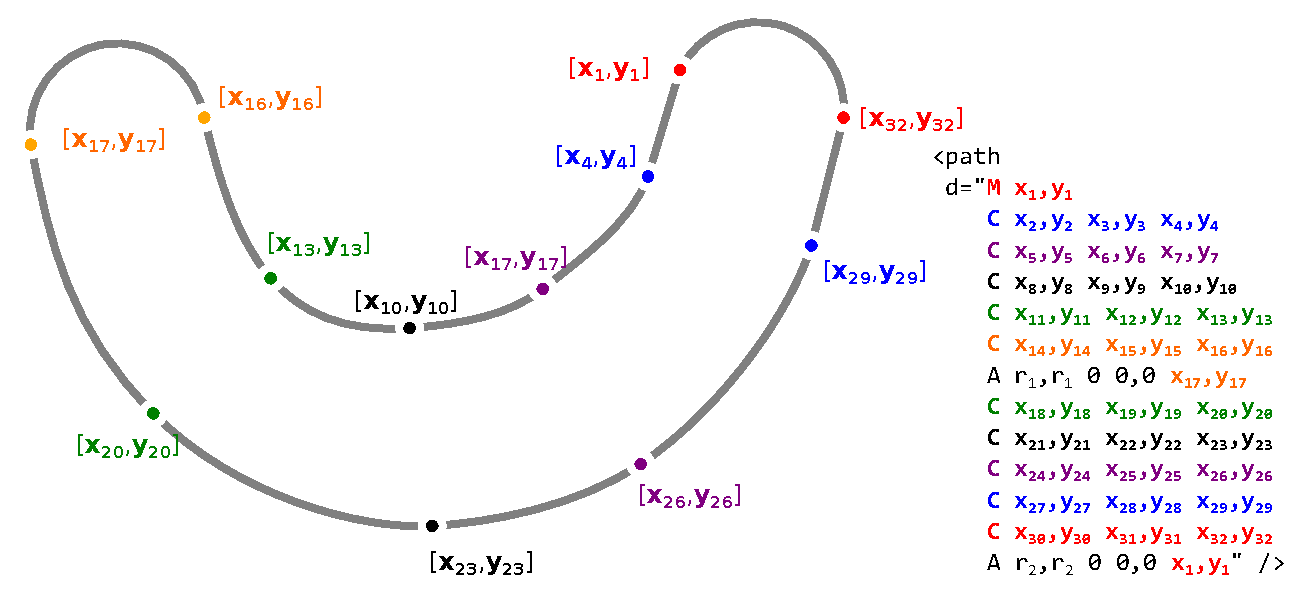
\includegraphics[width=130mm]{../img/path_serialization.eps}
		\caption{SVG path instructions corresponding to path segments\label{fig:parsing_path}}		
\end{figure}



\subsubsection{Audio capturing, processing and upload}

HTML5 provides only one way to access microphone data at the moment and it is through the \textit{getUserMedia API}~\cite{get_user_media}. \verb|navigator.getUserMedia| function prompts the user to for permission to use their audio input\footnote{\texttt|getUserMedia| function is also used to access webcam stream in other applications}.

If user's device has a connected microphone and user gives his permission to use his audio input, then a \verb|MediaStream| object is provided by the browser and from this time on audio can be processed. Error callback with \verb|MediaStreamError| instance as a parameter is called otherwise.

Current browsers implement \verb|ScriptProcessorNode| according to the W3C Working Draft from 10 October 2013 of \textit{Web Audio API}. Unfortunately, the \verb|ScriptProcessorNode| interface is deprecated in newer drafts of the specification and should be replaced with \verb|AudioWorkerNote| in the future\cite{mic_deprecated}. This new approach is not yet standardised, implemented and documented in web browsers. Both of these methods provide access to \verb|AudioBuffer| instance, which contains \textit{linear pulse-code modulation} (LPCM)\cite{wiki_pcm} sampled data from the microphone~\cite{mic_pcm}.

The \verb|Float32Array| buffer containing LPCM data gained from the AudioBuffer is converted to an \verb|Int16Array|. This reduces the amount of data that will be transferred over the Internet.



\subsubsection{High Resolution Timer}
To make the video look as good as possible, we need to store as precise data as possible. The \verb|Date.now()| function returns the number of milliseconds elapsed since 1 January 1970 00:00:00 UTC. The millisecond accuracy is satisfactory, but modern browsers provide even more accurate data via the \textit{High Resolution Time} via the \verb|window.performance.now()| function with the accuracy of microseconds. The \verb|window.performance.now()| function does not provide data related to current time, but the number of milliseconds elapsed since current page was loaded.

Video Screencast library cooses the most accurate timing function available by the web browser and uses it for making timestamps on recorded data or to control the playback of a screencast.




\section{User Interface}
Both the \verb|Player| and the \verb|Recorder| object instances receive an ID of an empty HTML element. User interface (UI) \nomenclature{UI}{User interface} HTML elements are created by the \verb|PlayerUI| and the \verb|RecorderUI| object instances. These objects create the whole UI, except for the blackboard (``canvas''). The blackboard is generated by an instance of \verb|DrawingStrategy| interface.

An instance of an object inheriting from \verb|PlayerUI| or \verb|RecorderUI| can be passed to a new instance of the tools in its constructor and override the default structure of the \verb|Player|, or \verb|Recorder| respectively.

UI object instance must map HTML elelements' events to the internal \verb|VideoEvents| and let the user control the recording or playback process.




\subsubsection{Input from pointing devices}

Detecting mouse movement and the state of its buttons is a very common task in web development. Users navigate through web pages mainly by clicking on hypertext links with their computer mouse. Therefore mouse events are well specified and work across all desktop web browsers and desktop platforms.

Unfortunately, the situation among other pointing devices other than computer mice is much less uniform. With the boom of smartphones and tablets, touchscreens are very common. Also computer graphics tablets are used by artists and many people use them when creating a Khan Academy style video.

\paragraph{Mouse input}
Event handler is passed the \verb|MouseEvent| object. The relevat information are the \verb|clientX| and \verb|clientY| properties, stating current mouse posititon relative to the position of the element it is attached to. 

\paragraph{Wacom Webplugin pen API}
The Wacom Webplugin pen API (WebPAPI) is a browser plugin interface for pen data access from all Wacom consumer and professional tablets. Unfortunatelly support for this plugin was discontinued by Chromium and Google Chrome~\cite{wacom_discontinued} and therefore it should not be relied on.

\paragraph{Touch Events API}
Touch Events API is an API for handling touch input from touch screens. The standard is proposed by Apple and is implemented across many platforms and in many mobile web browsers.

This API supports multiple touches at once, but this feature is not needed and neither implemented in this project. Unfortunately, this API provides no touch pressure information.

\paragraph{Pointer Events API}
Pointer Events API is an open API created by Microsoft. Its purpose is to unify the way mouse events, touch screen events, stylus and other (i.e. Kinect) similar ways into one API. This technology is implemented in Internet Explorer and will be also present in the final version of the Microsoft Edge browser. Firefox implements this API, but it is so far accessible only if a specific hidden flag is enabled. Google has announced the intent to also implement this functionality in upcoming releases of Google Chrome across all platforms.

This API also provides pressure information for pointing devices, that support this feature, including Wacom graphics tablets.















\section{Building the library}
\label{sec:building_the_library}

The library is written in TypeScript, which needs to be transpiled into pure JavaScript before it can be used. The theme uses the \textit{Less} CSS preprocesor, which also needs to be transpiled before it can be used. To simplify the process of building the library and its components, \textit{Gulp} streaming build system\footnote{http://gulpjs.com} is used.

\paragraph{Environment setup}
Source code of the project can be found either among the attached files, or in git repository \textit{https://github.com/simonrozsival/vectorvideo}. Copy or clone this code to your computer.

To be able to compile the library, it is necessary to install \textit{Node.js}\footnote{https://nodejs.org/} on your computer. After installing Node.js, install all dependencies of this project by running the \verb|npm install| command in the root directory of the project's source files. You must also install \textit{Gulp} globaly by running the \verb|npm install -g gulp| command.

\paragraph{Building library components}
Build all code by running \verb|gulp| command in the same directory. This will compile all TypeScript source files into JavaScript. You can then use the compiled and minified library located in \textit{./release/vector-screencast/vector-screencast.min.js} JavaScript file. Along with the library, a web worker file \textit{./release/workers/RecordingWorker.js}, which is necessary for audio recording. Default CSS theme of the player and recorder was compiled from LESS source to \textit{./release/themes/default/theme.min.css}.

A demo audio recording server was also compiled in this process and is available in the \textit{./release/audio-server/AudioServer.js} JavaScript file. This server can used in a Node.js program.

\begin{table}[ht]
	\centering
	  \begin{tabular}{L{4cm}L{9cm}l} %% the last column is a hack...
	  \hline
	  
	  \verb|gulp|             & Builds all parts of the project. & \\ \hline 
	  \verb|gulp release|	  &	Builds all parts of the project and places them in the \textit{/release} folder. Sources are minified and are ready for production use. & \\ \hline
	  \verb|gulp demo|		  &	Builds or sources for an example project. Sourcemaps are generated, so this demo is suitable for debugging. & \\ \hline
	  \verb|gulp doc|		  & Generates API documentation from the TypeScript source files and comments. & \\ \hline

	  \verb|gulp clean|       & Delete all the files that were created by the build.    & \\ \hline
	  \verb|gulp clean-release|       & Delete all the files that were created by the release build.    & \\ \hline
	  \verb|gulp clean-demo|       & Delete all the files that were created by the build of example project.    & \\ \hline
	  \verb|gulp clean-doc|       & Delete the generated API documentation.    & \\ \hline

	  \end{tabular}
	  \label{tbl:gulp}
	  \caption{Available gulp commands}
\end{table}


For details on how to use the library in your project, see chapter~\ref{ch:integration} on page~\pageref{ch:integration}.